\chapter{Home Automation}

Home automation, also known as domotics, has been a recurrent topic in Computer Science that
has become a reality in the last decades, thanks to the growth and decrease in the price of embedded
systems and wireless technologies, that have permitted to create distributed systems, the heart of this technology.

\bigskip
In this chapter, I am going to analyze this technology and its current state, including its implementation in commercial
products.

\section{What is home automation?}

Although science fiction has represented the idea of smart houses since the past century, including in them
an intelligence able to respond to all the dweller’s needs and desires, it has never felt as close to real world as today.

\bigskip
The basic idea of home automation is to employ sensors and control systems to monitor a dwelling, and accordingly 
adjust the various mechanisms that provide heat, ventilation, lighting, and other services. By more closely tuning the 
dwelling’s mechanical systems to the dweller’s needs, the automated "intelligent" home can provide a safer, more 
comfortable, and more economical dwelling.\cite{smarthouse98} For example, the automated system can determine 
the intensity and direction of the sunlight, and adequate the house according to its condition (which would include
closing the blinds and adjusting the air conditioner).

\bigskip
Unlike many may think, we don't actually need a very modern house, since advanced systems can be perfectly integrated 
in older, traditional buildings. This fact makes domotics a real possibility in every situation. In fact, the number of home 
automation systems installed in Europe is expected to reach around 29 million by 2019.\cite{statistaInstalled}

\begin{figure}
	\centering
	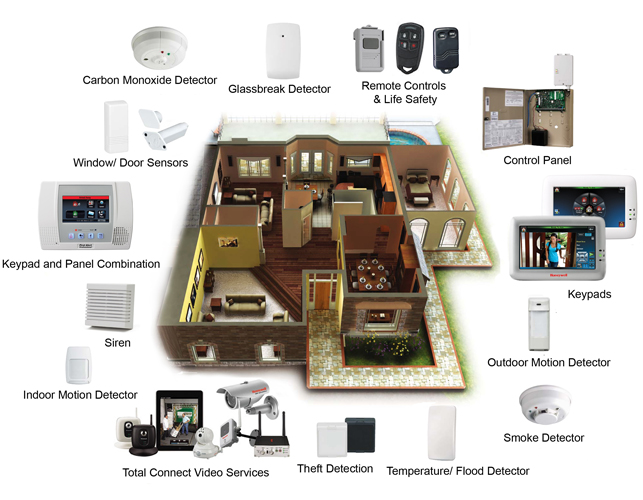
\includegraphics[width=0.9\textwidth]{images/Chapter_02/security.jpg}
	\caption{Example of a smart home with security-oriented devices}
	\label{fig:sh-security}
\end{figure}

\bigskip
There is not an exact point where we can set the beginning of the domotics as a real concept, but during the last century


\bigskip
What has made so popular the home automation is the broad range of benefits that it offers to their users.


